\documentclass[]{article}
\usepackage{lmodern}
\usepackage{amssymb,amsmath}
\usepackage{ifxetex,ifluatex}
\usepackage{fixltx2e} % provides \textsubscript
\ifnum 0\ifxetex 1\fi\ifluatex 1\fi=0 % if pdftex
  \usepackage[T1]{fontenc}
  \usepackage[utf8]{inputenc}
\else % if luatex or xelatex
  \ifxetex
    \usepackage{mathspec}
  \else
    \usepackage{fontspec}
  \fi
  \defaultfontfeatures{Ligatures=TeX,Scale=MatchLowercase}
\fi
% use upquote if available, for straight quotes in verbatim environments
\IfFileExists{upquote.sty}{\usepackage{upquote}}{}
% use microtype if available
\IfFileExists{microtype.sty}{%
\usepackage[]{microtype}
\UseMicrotypeSet[protrusion]{basicmath} % disable protrusion for tt fonts
}{}
\PassOptionsToPackage{hyphens}{url} % url is loaded by hyperref
\usepackage[unicode=true]{hyperref}
\hypersetup{
            pdftitle={Reliability and Validity of Physics Playground},
%            pdfauthor={Russell Almond, Jiawei Li, Zhichuan (Lukas) Liu, Seyedahmad Rahimi, Chen Sun and Seyfullah Tingir},
            pdfborder={0 0 0},
            breaklinks=true}
\urlstyle{same}  % don't use monospace font for urls
\usepackage[margin=1in]{geometry}
\usepackage{longtable,booktabs}
% Fix footnotes in tables (requires footnote package)
\IfFileExists{footnote.sty}{\usepackage{footnote}\makesavenoteenv{long table}}{}
\usepackage{graphicx,grffile}
\makeatletter
\def\maxwidth{\ifdim\Gin@nat@width>\linewidth\linewidth\else\Gin@nat@width\fi}
\def\maxheight{\ifdim\Gin@nat@height>\textheight\textheight\else\Gin@nat@height\fi}
\makeatother
% Scale images if necessary, so that they will not overflow the page
% margins by default, and it is still possible to overwrite the defaults
% using explicit options in \includegraphics[width, height, ...]{}
\setkeys{Gin}{width=\maxwidth,height=\maxheight,keepaspectratio}
\IfFileExists{parskip.sty}{%
\usepackage{parskip}
}{% else
\setlength{\parindent}{0pt}
\setlength{\parskip}{6pt plus 2pt minus 1pt}
}
\setlength{\emergencystretch}{3em}  % prevent overfull lines
\providecommand{\tightlist}{%
  \setlength{\itemsep}{0pt}\setlength{\parskip}{0pt}}
\setcounter{secnumdepth}{0}
% Redefines (sub)paragraphs to behave more like sections
\ifx\paragraph\undefined\else
\let\oldparagraph\paragraph
\renewcommand{\paragraph}[1]{\oldparagraph{#1}\mbox{}}
\fi
\ifx\subparagraph\undefined\else
\let\oldsubparagraph\subparagraph
\renewcommand{\subparagraph}[1]{\oldsubparagraph{#1}\mbox{}}
\fi

% set default figure placement to htbp
\makeatletter
\def\fps@figure{htbp}
\makeatother


\title{Reliability and Validity of Physics Playground}
%\author{Russell Almond, Jiawei Li, Zhichuan (Lukas) Liu, Seyedahmad Rahimi, Chen
%Sun and Seyfullah Tingir}
\author{Anne Alias and Ima Pseudonym}
\date{August 12, 2020}

\begin{document}
\maketitle

\section{\texorpdfstring{Calculating the Reliability and Validity of
\emph{Physics
Playground}}{Calculating the Reliability and Validity of Physics Playground}}\label{calculating-the-reliability-and-validity-of-physics-playground}

This paper presents a case study in calculating reliability and validity
for a cognitively diagnostic assessment of Physics using the game
\emph{Physics Playground}. The game is part of a game-based learning
system, so that students received instruction and feedback related to
Physics as they played. The game contained an internal measure of
Physics built with a Bayesian network. In the Spring of 2019, a field
trial involving 199 students played the game for 5 class periods and
also took an external measure of Physics understanding. This allows for
studying validity in the sense of correlation with the external measure.

\begin{figure}
\centering
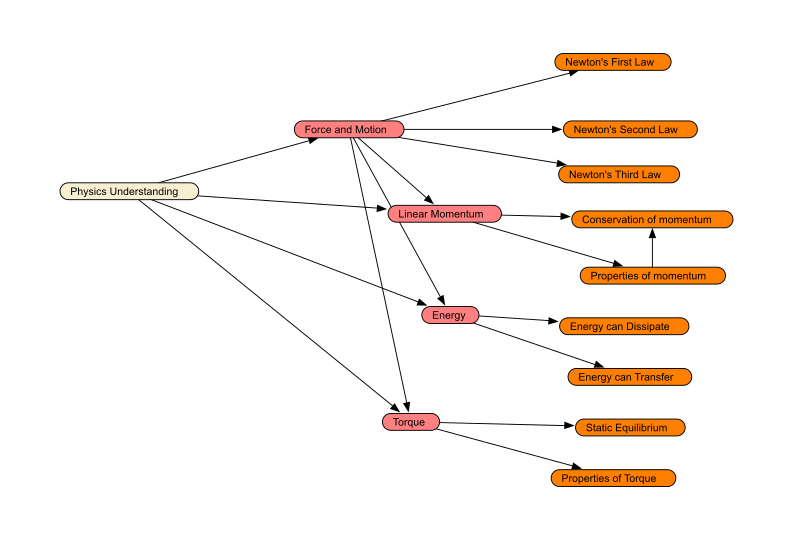
\includegraphics{PP_OrangeNodes_6.png}
\caption{Proficiency Model}
\end{figure}

The proficiency model for Physics used in \emph{Physics Playground}
consists of for high-level proficiencies (colored salmon in the figure)
and nine low-level proficiencies. Each of these nodes is represented by
an ordered variable with three states, \texttt{High}, \texttt{Medium}
and \texttt{Low}. The Bayes net provides a probability distribution over
these possible states for each node. There are thus three possible
statistics for each node that can be used as scores.

\begin{itemize}
\item
  \emph{Margin} -- This is a vector valued score with the probabilities
  for \texttt{High}, \texttt{Medium} and \texttt{Low}. The values will
  always add to 1. Note that any one of the three components can be used
  as a continuous score.
\item
  \emph{Mode} -- This is \texttt{High}, \texttt{Medium} or \texttt{Low}
  depending on which one has the highest probability. This is a
  categorical score.
\item
  \emph{EAP (Expected A Posteriori)} -- Assign the value +1 to
  \texttt{High}, 0 to \texttt{Medium} and -1 to \texttt{Low} and then
  calculate the expected value. This can be also expressed as
  \(\Pr(High) -\Pr(Low)\). The score runs from +1 (high) to -1 (low).
  (In the implementation, .97 and -.97 was used, so the actual scores do
  not every quite reach +1 or -1).
\end{itemize}

The EAP score is the one we primarily use for reporting. Its reliability
can be calculated using a split-half strategy and correlation. The
categorical score is an alternative, however, the same split-half
strategy can be used but this time with Cohen's kappa. An improved
categorical reliability can be calculated using the marginal scores
(Almond et al, 2015). The paper illustrates all three methods using the
data from the Spring 2019 field trial.

\subsection{\texorpdfstring{\emph{Physics
Playground}}{Physics Playground}}\label{physics-playground}

\emph{Physics Playground} (Shute et al, 2019) is a 2d Physics game that
consists of a number of levels. Each level is a puzzle in which the
player must use the principles of Newtonian Physics to move the ball to
the target balloon. Players win a gold trophy for an efficient solution
and a silver trophy for any solution. The game also records how long the
player took, how many objects were drawn and how many manipulations were
made.

Each game level has multiple observable outcome variables. All levels
had variables related to the trophy one and the time spent on the level.
Depending on the content of the level other variables were also
available, such as how many objects did the player create and how many
times did the player manipulate sliders which controlled gravity, air
resistance and other parameters. One of the advantages of working with
Bayesian networks is that they can be readily extended to multiple
observations per task.

Each game level was coded with a primary and secondary physics
competency (one of the nine low-level nodes in Figure 1). The levels
were also rated as to difficulty along two dimensions, \emph{Physics
Understanding} and \emph{Game Mechanics}. The former is related to the
difficulty of the items and the latter the discrimination. These were
used to build extended \(Q\)-matrixes for \emph{Physics Playground}.
These are stored in an
\href{https://docs.google.com/spreadsheets/d/16LcEuCspZjiBoZ3-Y1R3jxi1COXmh9vuTa9GwH1A_7Q/}{online
spreadsheet}. This Bayesian networks used for scoring are built directly
from this spreadsheet using the
\href{https://github.com/ralmond/Peanut}{Peanut} and the
\href{https://github.com/ralmond/EABN}{EABN} packages (Almond, 2020a,
b).

In the Fall 2020 study, players were randomized into three different
conditions which determined the order of the game levels. The players in
the \texttt{linear} condition saw the game levels in a fixed sequence,
players in the \texttt{adaptive} condition saw a sequence determined by
the scoring engine, and players in the \texttt{user\ control} condition
could choose which level they played next. Due to some technical
problems (now resolved) the adaptive condition did not show much
player-to-player variability. There were 75 game levels available to the
players, but most players completed substantially fewer. As the Bayesian
network can produce a score after the completion of any number of
levels, levels that were not attempted were simply not scored.

\subsection{Split-Half Reliabilities for EAP
Scores}\label{split-half-reliabilities-for-eap-scores}

The use of the \(Q\)-matrix and the difficulty indexes made it easy to
create matched half-tests. The forms were balanced according to (a) the
primary and secondary skills tapped (i.e., the \(Q\)-matrixes has
approximately the same structure as each other and the full test) as
well as physics understanding and game mechanics difficulty metrics.
They were also balanced as to whether the levels appeared early or late
in the default sequence, so that the number of not-reached levels should
be approximately the same in both forms.

It is a straightforward extension of the basic scoring algorithm for the
game to score the two half-forms. Player observables were stored in a
database. To score Form A, the observables from Form A levels were
marked as unprocessed and the assessment was rescored. The same trick
was applied to Form B. This produced a score on each of the 14 nodes of
the proficiency model from both forms. The correlation among those forms
in our measure of reliability.

For the Fall 2019 data, we got the following reliability numbers for the
EAP scores of the high-level nodes:

\begin{longtable}[]{@{}lr@{}}
\caption{Correlations between Form A and B sub-forms.}\tabularnewline
\toprule
Measure & Reliability\tabularnewline
\midrule
\endfirsthead
\toprule
Measure & Reliability\tabularnewline
\midrule
\endhead
Physics & 0.229\tabularnewline
Force and Motion & 0.135\tabularnewline
Linear Momentum & 0.080\tabularnewline
Energy & 0.456\tabularnewline
Torque & 0.139\tabularnewline
\bottomrule
\end{longtable}

These numbers are somewhat disappointing, however, they are also prior
to any refining or calibration of the network. Figure 2 show the
correlation for the Energy node which had the best performance, while
Figure 3 shows the correlation for Linear Momentum, which had the worst.

\begin{figure}
\centering
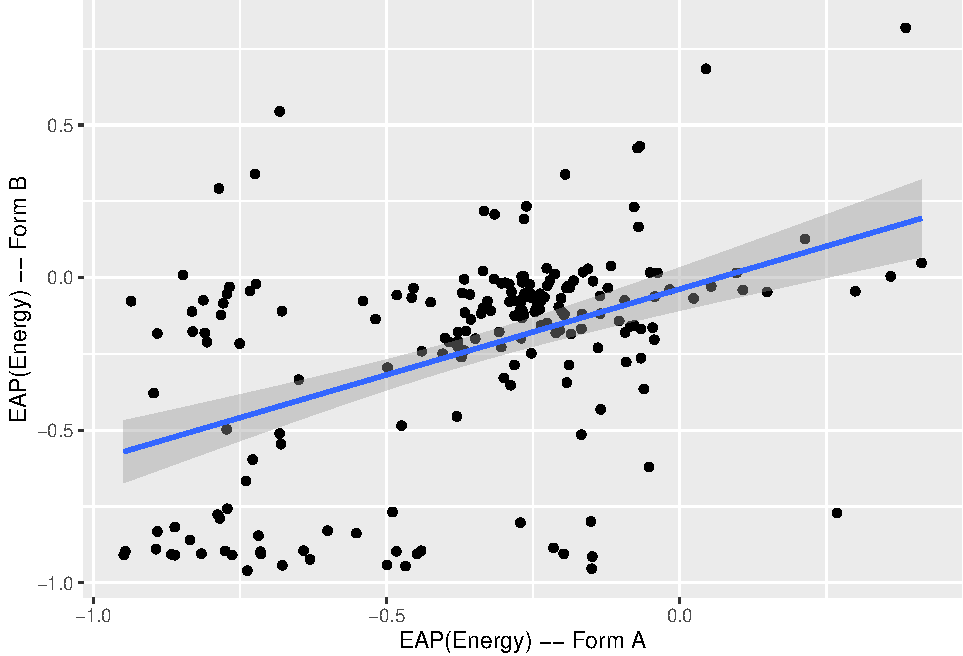
\includegraphics{PPReliablility_files/figure-latex/Energy-1.pdf}
\caption{Energy EAP scores, Forms A and B}
\end{figure}
\begin{figure}
\centering
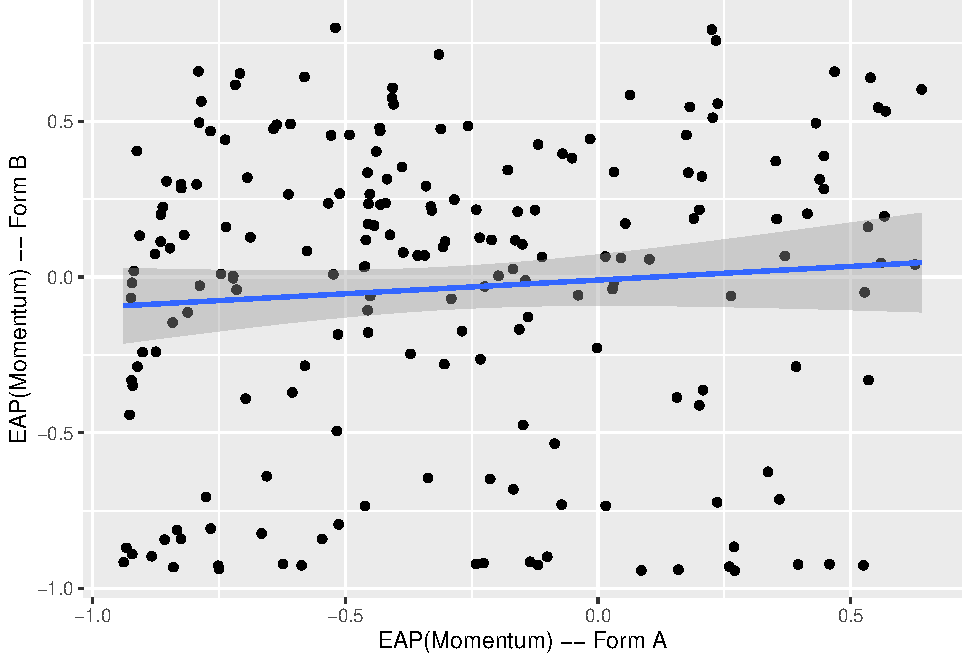
\includegraphics{PPReliablility_files/figure-latex/Momentum-1.pdf}
\caption{Linear Momentum EAP scores, Forms A and B}
\end{figure}

\subsection{Split-Half Consistency
Scores}\label{split-half-consistency-scores}

Turing to the modal scores, each student has a modal score from Form A
and Form B. We can make this to use a simple cross-tabulation as in
Table 2. Note that no student was classified as \texttt{High} in Physics
understanding. This indicates that the model is likely not well
calibrated. It also may be the case that the game is more difficult than
expected. (Games typically tend to be more difficult that conventional
assessments as the challenge is part of the game-like aspect.)

\begin{table}

\caption{\label{tab:Crosstab}Crosstabulation betwen Form A and Form B Modal scores.}
\centering
\begin{tabular}[t]{lrrr}
\toprule
  & H & M & L\\
\midrule
H & 0 & 0 & 0\\
M & 0 & 40 & 17\\
L & 0 & 89 & 53\\
\bottomrule
\end{tabular}
\end{table}

Cohen's kappa for this table is 0.05, which is disappointing. There are
a number of possible problems which could lead to such low results.

One known problem with the modal score is that it looses information. In
particular, a student who is on the borderline between \texttt{Medium}
and \texttt{Low} and a student who is on the borderline between
\texttt{Medium} and \texttt{High} can both be classified as
\texttt{Medium}. Looking using the marginal scores instead of the modal
scores gets around this problem. Consider a randomly chosen student.
That students marginal Physics scores on Form A and Form B are:

\begin{table}

\caption{\label{tab:FormAB124}Marginal Physics scores for Student 124, Form A}
\centering
\begin{tabular}[t]{rrr}
\toprule
High & Med & Low\\
\midrule
0.016 & 0.271 & 0.713\\
\bottomrule
\end{tabular}
\end{table}

\begin{table}

\caption{\label{tab:FormAB124}Marginal Physics scores for Student 124, Form B}
\centering
\begin{tabular}[t]{rrr}
\toprule
High & Med & Low\\
\midrule
0.015 & 0.673 & 0.313\\
\bottomrule
\end{tabular}
\end{table}

Taking the outer product of those two vectors, we get a probabilistic
confusion matrix:

\begin{table}

\caption{\label{tab:expAB124}Expected crosstabulation for Student 124}
\centering
\begin{tabular}[t]{lrrr}
\toprule
  & H & M & L\\
\midrule
H & 0.000 & 0.011 & 0.005\\
M & 0.004 & 0.183 & 0.085\\
L & 0.010 & 0.479 & 0.223\\
\bottomrule
\end{tabular}
\end{table}

Summing these across all 199 students yields a similar crosstab.

\begin{table}

\caption{\label{tab:ProbAB}Expected crosstabulation, all 199 students.}
\centering
\begin{tabular}[t]{lrrr}
\toprule
  & H & M & L\\
\midrule
H & 0.11 & 1.48 & 1.06\\
M & 2.84 & 42.65 & 29.66\\
L & 3.49 & 62.45 & 55.26\\
\bottomrule
\end{tabular}
\end{table}

Cohen's kappa remains unchanged at 0.05. This suggests that the problem
is with the assessment. Candidate issues include the lack of calibration
of the evidence and proficiency models, a task mix that is too
difficult, or a much smaller effective test length and students mostly
did not complete the whole assessment.

\subsection{Correlations with Pretest and
Posttest}\label{correlations-with-pretest-and-posttest}

As the Fall 2019 data collection involved a pretest and post-test, it is
possible to look at the correlation between the subscores from the
Bayesian network and the scores on the pretest and post-test items
designed to measure the same aspects of proficiency. In all cases, we
averaged the pretest and post-test to get alonger effect test length for
the criteriom measure, and did the correlation with the EAP scores from
the full form.

\begin{table}

\caption{\label{tab:Cormat}Correlation of Physics EAP score with whole pretest and posttest.}
\centering
\begin{tabular}[t]{lrrr}
\toprule
  & preScore & postScore & Physics\_EAP\\
\midrule
preScore & 1.000 & 0.698 & 0.226\\
postScore & 0.698 & 1.000 & 0.182\\
Physics\_EAP & 0.226 & 0.182 & 1.000\\
\bottomrule
\end{tabular}
\end{table}

While the pre-test and post-test hang together fairly well, the
correlation with the overall Physics score is disappointingly low. A
large part of the problem is likely the same issues causing low
reliability.

Turning to the four high-level nodes, we can also look at the
correlation with items on the pretest and post-test designed to tap
those aspects of proficiency. In this case, we add the pretest and
post-test scores together to make a longer instrument.

\begin{table}

\caption{\label{tab:Validity}Reliability (sub-form correlations) and Valitity (corrlation with pretest + posttest)}
\centering
\begin{tabular}[t]{lrr}
\toprule
Measure & Reliability & Validity\\
\midrule
Physics & 0.229 & 0.220\\
Force and Motion & 0.135 & 0.153\\
Linear Momentum & 0.080 & 0.061\\
Energy & 0.456 & 0.223\\
Torque & 0.139 & 0.174\\
\bottomrule
\end{tabular}
\end{table}

Again, these results are somewhat disappointing. However, the same steps
necessary to increase the reliability should increase the validity as
well.

\subsection{ECD and Validity}\label{ecd-and-validity}

Correlations with an external post-test are just one part of a complete
validity argument (Kane, 2006). Here, the evidence-centered design
methodology used in the game's construction (Shute et al, 2019) provides
a more qualitative approach to validity. In particular, the work with
experts in Physics pedagogy to validate the \(Q\)-matrix is an important
part of the validity argument. In particular, each game level represents
valued work in the domain of Physics.

That said, the reliabilities were disappointing, but looking at
reliabilities at the subscore rather than overall score level offers
insight into where and how the assessment can be improved. One obvious
first step is to do a calibration and move from the expert first guesses
in discrimination and difficulty to something which incorporates the
observed data. Another approach is to look closely at both the game
levels and the scoring models (particularly the choice of observables)
for the low information levels to see if improvements can be made.

Finally, the fact that different tasks are attempted by different
numbers of students adds a number of complications into the study of
reliability and validity. It is quite possible that the different
reliability of different measures is related to how many tasks students
usually attempted in those areas. In particular, a specific
reliability/validity study where the tasks are scheduled to provide a
more uniform exposure might improve the reliability measures. In this
scheduling, the system would cycle through all of the sub-domains, while
the activity selection algorithms for \emph{Physics Playground} have
attempted to deliberately stay within a sub-domain for an extended
period to maximize learning. This suggests that different data
collections may be needed for evaluating the effectiveness of
\emph{Physics Playground} as a learning environment and as a measurement
tool.

\subsection{Acknowledgements}\label{acknowledgements}

We would like to thank NSF for sponsoring the \emph{Physics Playground}
project (NSF \#1628937) and especially Val Shute, Principle
Investigator. Other member of the Physics Playground team (past and
present) include: Don Franceschetti, Renata Kamikabeya, Fengfeng Ke,
Adam LaMee, Xi Lu, Mathew Martens, Ginny Smith and Weinan Zhao.

\subsection{References}\label{references}

Almond, R. G., Mislevy, R. J., Steinberg, L. S., Yan, D. and Willaimson,
D. M. (2015). \emph{Bayesian Network in Educational Assessment}.
Springer.

Almond, R. G. (2020a) Peanut -- Software for Parameterized Bayesian
Networks. Computer software available from
\url{https://pluto.coe.fsu.edu/RNetica/Peanut.html} or
\url{https://github.com/ralmond/Peanut/}.

Almond (2020b) EABN -- Evidence Accumulation with Bayesian Networks.
Computer software available from \url{https://pluto.coe.fsu.edu/Proc4/}
or \url{https://github.com/ralmond/EABN/}.

Kane, M. T. (2006). Validation. \emph{Educational Measurement (4th
Edition).} American Council on Education/Praeger, 2006.

Shute, V. J., Ke, Fengfeng, Almond, Russell G., Rahimi, S., Smith, G.
and Lu, X. (2019). How to Increase Learning while not Decreasing the Fun
in Educaitonal Games. \emph{Learning Science: Theory, Research and
Practice.} 327--357.

\end{document}
